\chapter{CryptoNight e Resistenza agli ASIC}
\section{Protocollo di consenso}
In una rete blockchain pubblica, nessuna singola entità detiene esclusivamente l'autorità di verificare e validare le transazioni, in quanto un avversario potrebbe falsificare una catena di blocchi con transazioni false e propagare la blockchain fasulla nella rete. 
Pertanto, un componente fondamentale delle reti blockchain è il protocollo di consenso, che consiste in un insieme di regole e procedure utilizzate per raggiungere un accordo comune, tra tutti i nodi partecipanti alla rete, sullo stato della blockchain.

\subsection{Proof Of Work (PoW)}
Uno dei protocolli di consenso più utilizzati è il Proof-of-Work (PoW) che si basa sul dimostrare di aver svolto uno sforzo computazionale per creare un blocco che soddisfa il protocollo di consenso. 
Questo processo, che porta ad avere un nuovo blocco valido da inserire nella blockchain, prende il nome di \textit{mining}.
In base alla blockchain considerata, il minatore che ha inserito il blocco può raccogliere le ricompense predefinite e/o le commissioni delle transazione contenute in tale blocco.

L'idea iniziale era che ogni partecipante potesse unirsi al processo di mining utilizzando le proprie risorse computazionali. 
In questo modo, un avversario per violare il protocollo PoW, deve necessariamente possedere una potenza di calcolo superiore a quella aggregata di tutti gli altri partecipanti al mining (attacco del 51\%). 
Tuttavia, questa minaccia inizia a diventare sempre più reale a causa della diffusione di miner basati su circuiti integrati specifici. 


\section{Mining: CPU vs GPU vs FPGA vs ASIC}
Tra le tecnologie maggiormente usate per il mining possiamo distinguere: ASIC (Application-Specific Integrated Circuits), FPGA (Field-Programmable Gate Arrays), GPU (Graphics Processing Units), e CPU (Central Processing Units). 

Ognuna di queste tecnologie viene impiegata per scopi precisi e presenta delle limitazioni rispetto alle altre.
Pertanto, dato che scegliere l'una piuttosto che l'altra comporta differenze in termini di efficienza e costi, è importante avere un idea generale delle loro differenze.

\begin{itemize}
    \item Le \textbf{CPU}, le "generaliste del gruppo" presenti in ogni personal computer, offrono grande flessibilità, in quanto sono in grado di gestire un'ampia gamma di compiti a scapito dell'efficienza specializzata riscontrabile nelle altre tecnologie.
    \item Le \textbf{GPU}, inizialmente sviluppate per il rendering grafico, hanno trovato applicazioni diverse grazie alla loro capacità di elaborazione parallela, dimostrandosi strumenti potenti nei calcoli ad alta intensità di dati.
\end{itemize}

Nel contesto del mining di criptovalute, CPU e GPU sono state le prime scelte, ma con l'aumento della "concorrenza", ASIC e FPGA come soluzioni più efficienti.

\begin{itemize}
    \item Gli \textbf{FPGA (\textit{Field Programmable Gate Arrays})} possono implementare una vasta gamma di funzioni circuitali, in quanto sono fondamentalmente dispositivi modificabili fisicamente per creare lo specifico circuito elettronico che si desidera. 

    Poiché devono essere versatili, i componenti presenti internamente hanno molte caratteristiche che non vengono sfruttate. 
    Di conseguenza, nonostante possano raggiungere prestazioni superiori ad un computer general purpose, non sono ottimizzati per il consumo energetico e la velocità in un'applicazione specifica come quella del mining. 

    \item Un \textbf{ASIC (\textit{Application-specific integrated circuit})} è simile ad un FPGA in quanto utilizza un circuito elettronico cablato per eseguire una funzione computazionale. 
    A differenza di un FPGA, un ASIC può essere ottimizzato per il consumo energetico ridotto, la velocità o una combinazione di entrambi, comportandosi quindi sempre meglio di un FPGA programmato per fare lo stesso lavoro. 
    
    Gli svantaggi di un ASIC sono il costo di ingresso elevato ed il complesso processo di progettazione necessario per il loro sviluppo.

    La non modificabilità degli ASIC è il loro punto di forza in termini di consumo energetico e velocità, ma è anche una loro criticità. 
    Essendo progettati per eseguire un compito specifico, non possono essere adattati o aggiornati per eseguire funzioni diverse da quelle per cui sono stati progettati. 
    Pertanto, se una blockchain dovesse cambiare l'algoritmo di mining, gli ASIC progettati per minare su essa, diventerebbero obsoleti ed inefficaci poiché non modificabili.
\end{itemize}

Nonostante quest'ultima problematica, gli ASIC restano la minaccia più grande alle blockchain, in quanto offrono prestazioni superiori e un consumo energetico ottimizzato specificamente per il mining. 
Con il predominio di questi circuiti integrati, appositamente progettati per il calcolo di specifici PoW, la decentralizzazione delle reti blockchain e la looro integrità è messa a rischio. 



\subsubsection{Caso Bitcoin}
Osservando il grafico in Figura \ref{fig:btc-hashrate}, si può vedere come l'hashrate aggregato della rete Bitcoin, ovvero il numero di hash che vengono prodotti globalmente al secondo, è aumentato drammaticamente.

\begin{figure}[h!]
    \centering
    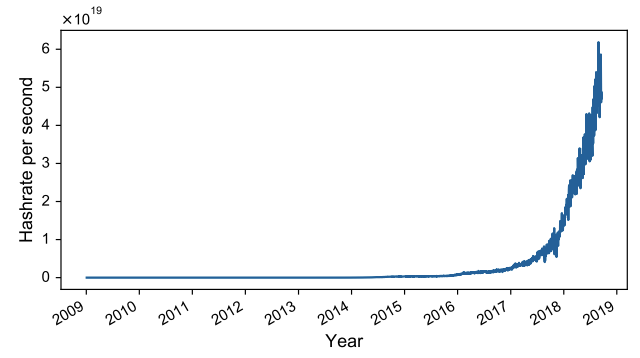
\includegraphics[width=0.55\linewidth]{images/bitcoin_hashrate.png}
    \caption{Hashrate della blockchain Bitcoin \cite{asic1}}
    \label{fig:btc-hashrate}
\end{figure}

La motivazione riconducibile a ciò è proprio l'avvento degli ASIC e la loro partecipazione al mining di Bitcoin.

Il mining basato su ASIC ha creato un picco barriera all’ingresso per il grande pubblico perché, chi interessato a minare, dovrebbe investire in attrezzature speciali per partecipare a tale processo.
A causa di ciò, come precedentemente accennato, le poche entità in grado di investire e mantenere un grande volume di ASIC potrebbero assumere il controllo della rete.
Pertanto, il mining basato su ASIC è maggiore vulnerabile all’attacco del 51\%. 


A partire da settembre 2018, i mining-pool\footnote{\textbf{Mining-pool}: minatori di criptovalute che uniscono le loro risorse per estrarre criptovalute e aumentare le probabilità di ottenere la ricompensa di un blocco} Bitcoin BTC.com e Antpool, che sono gestiti dalla stessa azienda che produce gli ASIC per la blockchain bitcoin, rappresentano oltre il 30\% del potere (hashrate) nella rete Bitcoin. 


\section{Introduzione alle PoW ASIC-resistant}
Al fine di scoraggiare l'uso di sistemi basati su ASIC per il mining, sono stati proposti diversi meccanismi PoW ASIC-resistant.
I principali algoritmi di questo tipo possono essere divisi in: PoW Multi-hash, PoW Memory-hard e PoW Programmatico.

\subsection{PoW Multi-hash}
A differenza dell'algoritmo PoW di Bitcoin che utilizza solo un tipo di funzione hash, gli algoritmi PoW Multi-hash impiegano più funzioni hash per calcolare la validità del blocco. Queste funzioni hash vengono applicate all'intestazione del blocco in una sequenza, che può essere fissa o determinata dinamicamente per ogni blocco. 
Alcuni degli algoritmi PoW multi-hash più famosi sono: \textit{X11, X14, X17, X11EVO, X16S, X16R, Quark} e \textit{TimeTravel}.

Nella ricerca scientifica di Cho, dal titolo "\textit{ASIC-Resistance of Multi-Hash Proof-of-Work Mechanisms for Blockchain Consensus Protocols}" \cite{asic1}, è stato dimostrato come gli algoritmi multi-hash non hanno una significativa differenza da altri meccanismi PoW semplici.
Inoltre, nonostante gli algoritmi di questa categoria siano spesso definiti ASIC-resistance, alcuni di loro sono già stati rotti da sistemi ASIC.
Mentre, per quanto riguarda gli algoritmi rimanenti, non è stato mai dimostrato se siano veramente resistenti agli ASIC o se semplicemente non sono ancora stati progettati ASIC specifici per essi, magari in quanto impiegati in reti piccole dal basso valore economico.

Dati i risultati ottenuti, nel paper si suggerisce di optare per l'impiego di altri meccanismi ASIC-resistant per scoraggiare effettivamente il mining basato su ASIC.


\subsection{PoW Memory-hard}
Sebbene gli ASIC offrano una maggiore efficienza computazionale rispetto alle piattaforme di calcolo general-purpose, sono solitamente limitati in termini di memoria.
    
In un algoritmo PoW Memory-hard, il processo di mining richiede l'utilizzo di grandi quantità di memoria per importare dati complessi e calcolarne l'hash.
Una computazione in questi algoritmi richiederà il recupero di dati casuali da un grande set di dati. 
La dimensione dell'insieme sarà sufficientemente grande da rendere difficile la progettazione di un ASIC che memorizzi tutto in una memoria on-chip.

Gli algoritmi PoW memory-hard più conosciuti sono: \textit{Ethash} di Ethereum, \textit{Scrypt} e \textit{CryptNight}. 

%\begin{itemize}
    %\item In Ethash, il dataset è di diversi gigabyte e aumenta continuamente di dimensioni. 
    %La posizione dei dati che devono essere recuperati per ogni computazione PoW con nonce diversi viene determinata durante la computazione, il che significa che non è fattibile pre-caricare i dati richiesti o raggruppare più nonce che accedono alla stessa posizione del dataset. 
    %Pertanto, l'hashrate effettivo sarebbe limitato dalla larghezza di banda dei dati off-chip disponibile sulla piattaforma.
    
    %\item In Cryptonight, invece, ci si basa su una grande tabella di dati in memoria, soggetta a frequenti aggiornamenti e sulla funzione di hashing Keccak calcolata sulla memoria cache. 
%\end{itemize}


\subsection{PoW Programmatico}
Infine, una delle nuove direzioni per meccanismi PoW resistenti è aumentare la diversità delle computazioni. 
Nell'approccio PoW Programmatico, il processo di mining coinvolge l'esecuzione di un programma che cambia frequentemente. 
Ad esempio, aggiungendo come parte della computazione un pool di funzioni matematiche o un programma generato casualmente. 

Questo rende difficile per gli ASIC ottimizzare il mining, poiché dovrebbero essere riprogrammati ogni volta che il programma cambia.
Sarebbe impraticabile costruire moduli hardware specializzati che mirino a ciascuna delle possibili attività di calcolo.  

Questo tipo di meccanismi PoW sono in fase di studio e non sono ancora stati utilizzati per la realizzazione di una vera e propria blockchain.


\section{CryptoNight Hash Function}
Come descritto precedentemente per gli algoritmi PoW memory-hard, i processori specializzati quali ASIC e FPGA hanno un vantaggio minimo rispetto alle CPU e GPU a causa della complessità degli algoritmi e dell'elevato costo della memoria. 

Ad esempio, nella blockchain Ethereum l'algortimo di consenso è \textit{Ethash}. L'Antminer E3 sviluppato per minare su Ethereum ha un hash rate di 190 MH/s, che è solo 2 volte più veloce della GPU V100, a fronte di un consumo energetico 3 volte superiore.

\subsection{Algoritmo CryptoNight}
Un altro algoritmo di PoW molto conosciuto, classificabile come memory-hard, è CryptoNight. 
Tale algoritmo è compreso nel protocollo di consenso CryptoNote rilasciato nel 2013 e cerca di offrire un'\textbf{elevata dipendenza da CPU}, resistendo ad ASIC, FPGA e GPU.

Si ricordi che le CPU moderne possono essere costituite da un massimo di qualche decina di core e possono utilizzare più livelli di cache per migliorare la velocità di accesso alla memoria. 
Nello specifico, le cache L1 e L2 sono private per ogni core, mentre la cache L3 è condivisa da tutti i core. 

CryptoNight contiene un ciclo memory-hard, che esegue una sequenza di letture e scritture casuali in una piccola area di memoria da 2MB, chiamata \textit{scratchpad}. 
Questo ciclo è stato progettato per funzionare in modo efficiente sulle CPU perché lo scratchpad è dimensionato per adattarsi alla \textbf{cache L2} della CPU. 

L'algoritmo CryptoNight si compone di tre fasi principali: inizializzazione dello scratchpad, il memory-hard loop e calcolo del risultato.

\subsubsection*{Fase 1: Inizializzazione dello scratchpad}
Utilizzando la funzione Keccak (SHA3) vengono generati 200 byte. 
\begin{itemize}
    \item I primi 32 byte (0-31) vengono utilizzati come chiave AES-256. 
    \item I successivi 128 byte  (64-191), vengono divisi in otto blocchi di 16 byte ciascuno, e ciascuno di questi otto blocchi viene cifrato per 10 round AES utilizzando la chiave AES-256. 
    \item Il risultato della cifratura viene memorizzato come i primi 128 byte della memoria dello scratchpad. Successivamente, viene eseguita iterativamente la cifratura AES sui 128 byte correnti dello scratchpad e il risultato viene aggiunto come i successivi 128 byte nello scratchpad. 
    \item Questo processo continua fino a quando l'intero scratchpad è riempito.
\end{itemize}
    
\subsubsection*{Fase 2: Memory-hard loop}
Come elencato nell'Algoritmo XX e illustrato nella Figura \ref{fig:cryptonight-loop}. 
\begin{itemize}
    \item Sia A che B sono interi a 16 byte e vengono inizializzati con il risultato XOR dei byte da 0 a 31 e da 32 a 63 generati utilizzando la funzione Keccak. 
    \item Questi interi vengono quindi utilizzati come indirizzi nello scratchpad analizzando i 21 bit meno significativi. 
    Si legge il valore S[A] nello scratchpad usando A come indirizzo e si esegue la crittografia AES di S[A] con A per ottenere il risultato C. 
    \item Successivamente si esegue lo XOR su B e C e si riscrive il risultato XOR in S[A]. Si usa poi C come indirizzo, si legge S[C] in D, si moltiplicano C e D, si aggiunge il risultato della moltiplicazione ad A e si memorizza A in S[C].
    \item Infine, si ottiene il risultato XOR di A e D come nuovo A, e C come nuovo B, e si utilizeranno il nuovo A e B all'iterazione successiva. 
\end{itemize}

\begin{figure}[h!]
    \centering
    \makebox[\textwidth][c]{
    
        \begin{minipage}{0.5\linewidth}
            \centering
            \begin{algorithm}[H]
            \caption{}
            \begin{algorithmic}[1]
            \Require Integer $A$, $B$, Scratchpad memory $S$
            \Ensure Modified scratchpad memory $S$
            \For{$i \leftarrow 1$ to $524288$}
                \State $C \leftarrow \text{AES}(S[A], A)$
                \State $S[A] \leftarrow \text{XOR}(B, C)$
                \State $D \leftarrow S[C]$
                \State $A \leftarrow \text{ADD}(A, \text{MUL}(C, D))$
                \State $S[C] \leftarrow A$
                \State $A \leftarrow \text{XOR}(A, D)$
                \State $B \leftarrow C$
            \EndFor
            \end{algorithmic}
            \end{algorithm}
        \end{minipage}
        
        \hspace{0.05\linewidth}
        
        \begin{minipage}{0.45\linewidth}
            \centering
            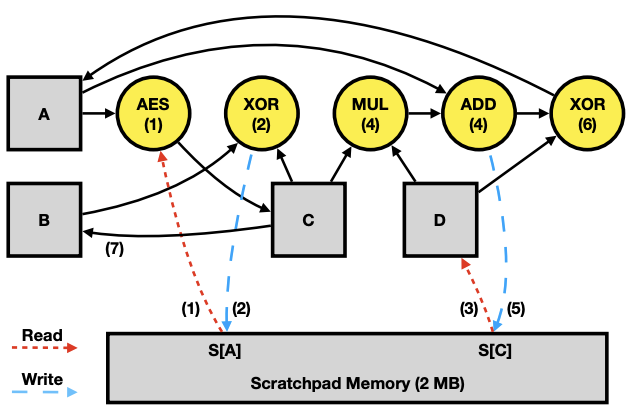
\includegraphics[width=\linewidth]{images/cryptonight.png}
        \end{minipage}
    }
    \caption{Memory-Hard loop dell'algoritmo CryptoNight. \cite{asic_memory_hard}}
    \label{fig:cryptonight-loop}
\end{figure}

Poiché l'output della crittografia AES è casuale, non è possibile prevedere l'indirizzo, quindi il ciclo non può essere parallelizzato. Il ciclo contiene 524.288 iterazioni, quindi verrà eseguita una sequenza di 2 milioni di letture e scritture casuali complessive sullo scratchpad.

\subsubsection*{Fase 3: Calcolo del risultato} 
Similmente al primo passo, i byte da 32 a 63 del risultato iniziale di Keccak vengono utilizzati come chiave AES-256 e i byte da 64 a 191 vengono crittografati con il contenuto della memoria scratchpad, 128 byte alla volta. 

Successivamente, la permutazione Keccak viene eseguita una volta sul risultato della crittografia. A seconda dei due bit meno significativi del primo byte del risultato Keccak, verrà scelto uno dei quattro algoritmi di hash: BLAKE-256, Groestl-256, JH-256 o Skein256. L'algoritmo di hash selezionato viene applicato sul risultato Keccak per produrre l'output finale di CryptoNight.

Con CryptoNight come protocollo di consenso della blockchain, agli utenti che richiedono di aggiungere un nuovo blocco verrà richiesto di eseguire ripetutamente l'algoritmo CryptoNight fino a trovare un nonce $n$ tale che $H(n||b) \times d < 2^{256}$, dove $H$ è la funzione di hash CryptoNight, $b$ è il contenuto del nuovo blocco e $d$ è la difficoltà. 

Quando un nuovo blocco viene trasmesso alla rete blockchain, il validatore eseguirà la funzione di hash CryptoNight sul nuovo blocco per verificare se il valore di hash del nuovo blocco sia effettivamente inferiore alla soglia data.

L'algoritmo Cryptonight non è considerato un algoritmo multi-hash nel senso tradizionale. Anche se potrebbe utilizzare più passaggi di hash all'interno del suo processo di computazione, la sua caratteristica distintiva è la sua natura memory-hard . 



\subsubsection{Risultati sperimentali}
Nel paper intitolato "\textit{Evaluating Memory-Hard Proof-of-Work Algorithms on Three Processors}" \cite{asic_memory_hard}, Feng e Luo confrontano tra loro \textit{CryptoNight}, \textit{Ethash}, \textit{Hashcash} e \textit{Cuckoo} su CPU, GPU e KNL, giungendo alla conclusione che la Memory-Hardness può essere raggiunta sfruttando la latenza o la bandwith.

I compiti che dipendono dalla latenza sono più adatti per CPU, grazie alla loro gerarchia di cache ben sviluppata. 
Al contrario, i compiti che richiedono una grande larghezza di banda possono sfruttare appieno il potenziale delle GPU.

Nel caso di studio, CryptoNight implementa una resistenza alla memoria mediante la latenza, sfruttando il tempo di accesso alla memoria per rendere più difficile la creazione di hardware specializzato.

Tuttavia, come seconda considerazione, viene specificato che, poiché i processori si stanno evolvendo rapidamente, gli algoritmi di Proof-of-Work dovrebbero essere adattabili e flessibili affinché le loro proprietà possano essere mantenute il più a lungo possibile. 



\subsection{La vittoria degli ASIC su CryptoNight}
CryptoNight rimase immune agli ASIC per un lungo periodo. Tuttavia, a partire dal 2018 vennero annunciati diversi modelli di ASIC per CryptoNight (Bitmain, Baikal e Halong Mining), capaci di raggiungere un hashrate superiore ai 200 KH/s.


\subsubsection{Bitmain}
Il 15 marzo 2018, Bitmain, un'azienda cinese, ha annunciato l'Antminer-X3, un ASIC progettato appositamente per il mining di criptovalute basate su CryptoNight. Secondo le specifiche riportate sul sito di Bitmain, l'X3 ha un tasso di hash totale di 220 kH/s e un consumo energetico di 465W.

È interessante notare la risposta su Twitter del responsabile del progetto Monero all'epoca, Riccardo Spagni, il quale sottolinea l'inefficacia dell'Antminer-X3 per la blockchain di Monero (Figura \ref{fig:Antminer-X3}).
Al tempo Monero utilizzava come PoW proprio CryptoNight, tuttavia come parte del suo protocollo blockchain adotta regolarmente hard fork pianificati e di emergenza al fine di mitigare qualsiasi potenziale minaccia derivante dagli ASIC.

% https://www.getmonero.org/2018/02/11/PoW-change-and-key-reuse.html

\begin{figure}[h!]
    \centering
    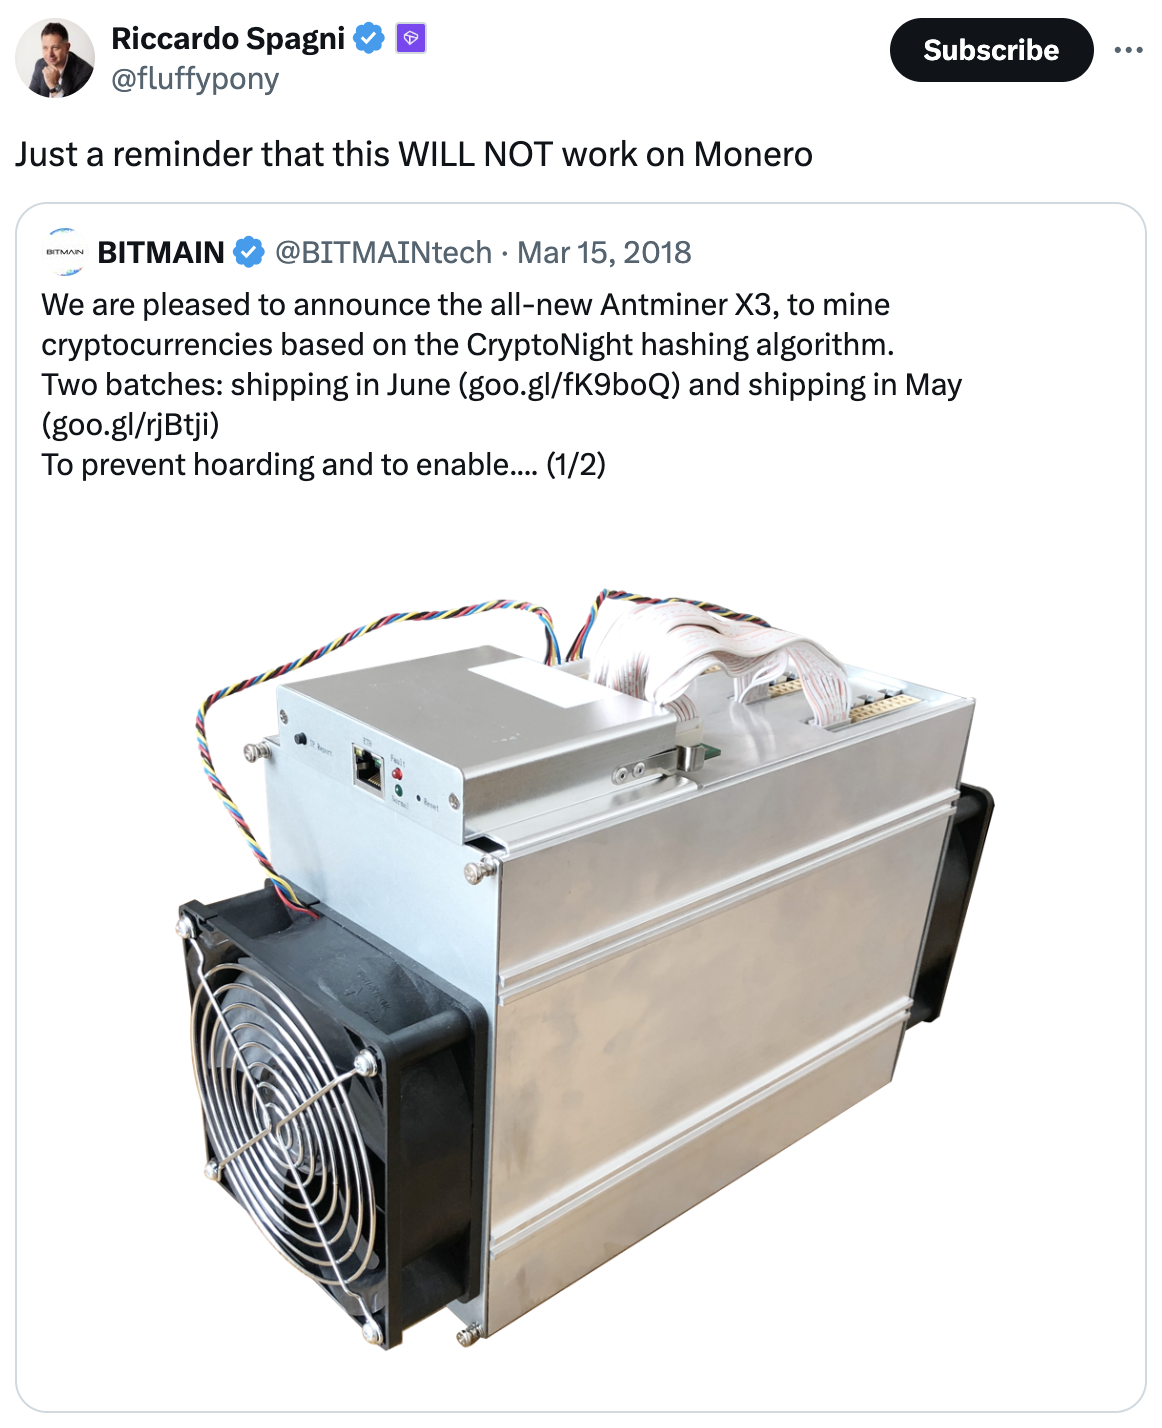
\includegraphics[width=0.45\linewidth]{images/Antminer-X3.png}
    \caption{Modello Antminer-X3 (Bitmain)}
    \label{fig:Antminer-X3}
\end{figure}

La strategia adottata da Monero gli conferisce immunità agli ASIC come l'X3 e quelli che presentati nelle prossime sezioni. 
Tuttavia, tali dispositivi rimangono utili per il mining di altre criptovalute basate su CryptoNight, come Bytecoin, Dinastycoin, Karbo e vecchie fork di Monero, che non implementano misure simili.


% TODO: vedere formattazione delle pagine prima di rimuovere
\subsubsection{Baikal}
Anche la società russa Baikal Mining ha reagito prontamente, rilasciando un primo modello meno potente nello stesso mese del concorrente cinese e un secondo modello più performante alcuni mesi dopo.
Entrambi gli ASIC sono in grado di minare gli algoritmi CryptoNight e CryptoNight-Lite.

\begin{itemize}
    \item[(a)] Modello BK-N, rilasciato nel marzo 2018 con un hashrate massimo di 80 kH/s ed un consumo di 120W (Figura \ref{fig:Baikal BK-N}),
    \item[(b)] Modello BK-N240, rilasciato nel maggio 2018 con un hashrate massimo di 480 kH/s ed un consumo di 650W (Figura \ref{fig:Baikal N240}).
\end{itemize}

\begin{figure}[h!]
    \centering
    \begin{subfigure}[b]{0.15\linewidth}
        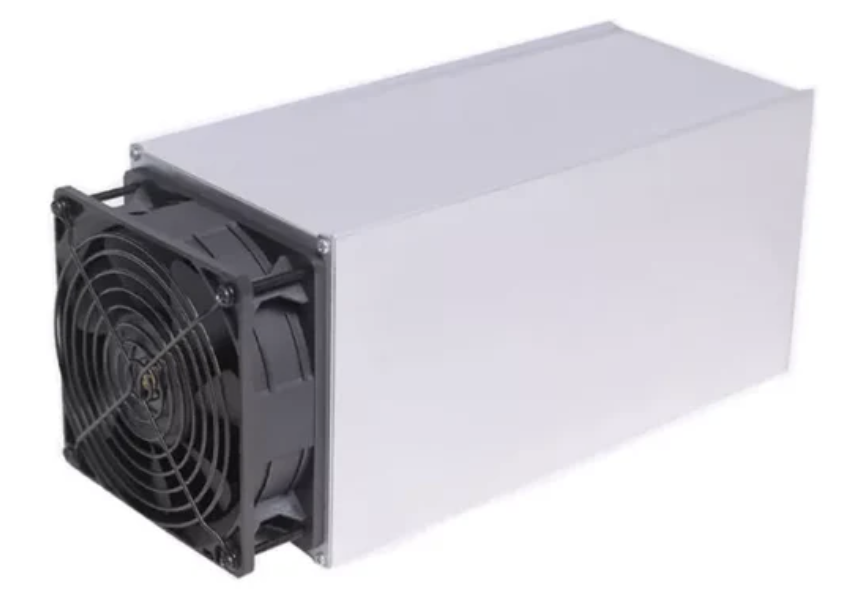
\includegraphics[width=\linewidth]{images/Baikal BK-N.png}
        \caption{}
        \label{fig:Baikal BK-N}
    \end{subfigure}
    \hspace{1.5cm}
    \begin{subfigure}[b]{0.15\linewidth}
        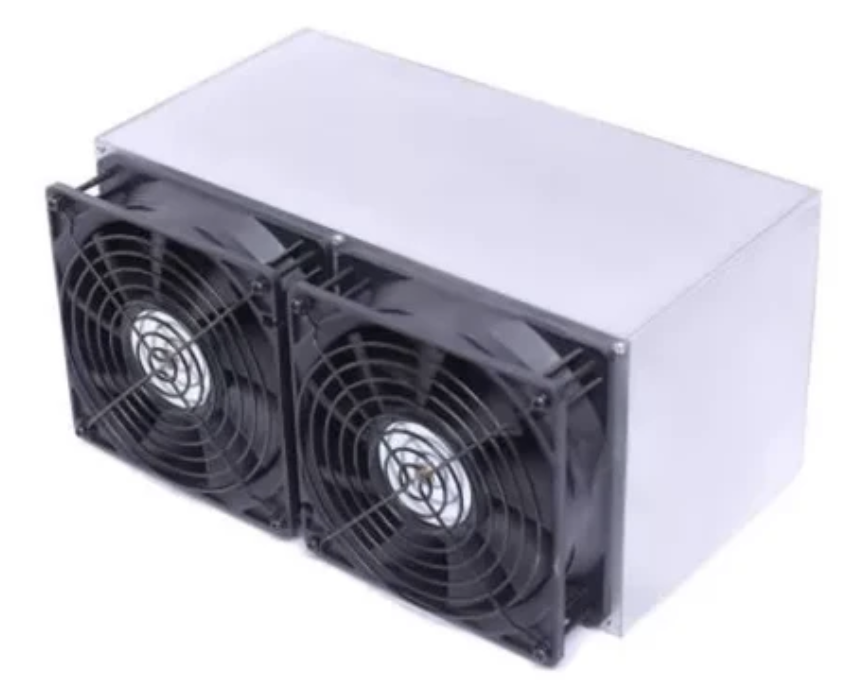
\includegraphics[width=\linewidth]{images/Baikal N240.png}
        \caption{}
        \label{fig:Baikal N240}
    \end{subfigure}
    \caption{Modelli ASICS BK-N e BK-N240 (Baikal)}
    \label{fig:Baikal miners}
\end{figure}


\subsubsection{Halong Mining}
Con un mese di ritardo, nell'Aprile 2018, anche l'azienda statunitense Halong Mining ha rilasciato il suo Modello DragonMint X2, in grado di minare l'algoritmo CryptoNight con un hashrate massimo di 248 kH/s e un consumo energetico di 490W.

\begin{figure}[h!]
    \centering
    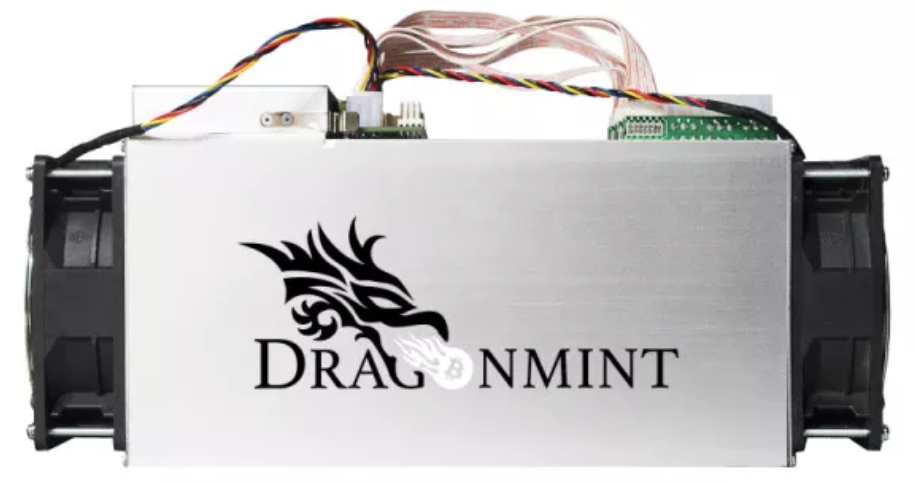
\includegraphics[width=0.2\linewidth]{images/DragonMint X2.png}
    \caption{Modello ASICS DragonMint X2 (Halong Mining)}
\end{figure}

